\documentclass{beamer}
\usepackage{amsfonts,amsmath,oldgerm}
\usepackage{ctex, hyperref}
\usepackage[T1]{fontenc}
\usepackage{booktabs}
\usepackage{hyperref}
\hypersetup{
    %colorlinks=true,
    %linkcolor=black,
    %filecolor=black,      
    urlcolor=blue,
    pdftitle={Bayesian Statistics Presentation},
    pdfpagemode=FullScreen,
    }
\usepackage[backend=biber, style=apa, sorting=ynt]{biblatex}
\addbibresource{ref.bib}
\usepackage{latexsym,amsmath,xcolor,multicol,booktabs,calligra}
\usepackage{graphicx,pstricks,listings,stackengine}

\usetheme{sintef}

\newcommand{\testcolor}[1]{\colorbox{#1}{\textcolor{#1}{test}}~\texttt{#1}}

\usefonttheme[onlymath]{serif}

\titlebackground*{assets/background.png}

\newcommand{\hrefcol}[2]{\textcolor{cyan}{\href{#1}{#2}}}

\title{Which factors are contributing to Greenhouse gas emissions in Italy?}
\subtitle{Bayesian analysis}
\institute{Università degli studi di Milano}
\author{David Fernandez, Alessia Leo Folliero}
\date{May 12, 2023}

\begin{document}
\maketitle


\begin{frame}
    \tableofcontents[sectionstyle=show,subsectionstyle=show/shaded/hide,subsubsectionstyle=show/shaded/hide]
\end{frame}

\section{Introduction}

\begin{frame}{Research question}
\Huge{Which factors are contributing to Greenhouse gas emissions in Italy?}
\end{frame}

\begin{frame}{What are Greenhouse gases? \footnote{ \emph{Greenhouse gas emissions:} \url{https://bit.ly/423jXKk}}}
  \begin{figure}[H]
    \centering
    \includegraphics[width=0.8\textwidth]{pic/Intro1.png}
    %\caption{Greenhouse gases composition}
    \label{fig:Fig1}
\end{figure}
\end{frame}


\begin{frame}{How do they affect the climate? \footnote{ \emph{The consequences of the greenhouse effect: from desertification to floods:} \url{https://bit.ly/40QZcjq}}}
    \begin{itemize} %[<+-| alert@+>]
        \item increase in temperature
        \item increased frequency of severe storms
        \item increases in droughts
        \item warming rising ocean
    \end{itemize}
\end{frame}

\section{Data description}

\begin{frame}{Data}
    \begin{itemize} %[<+-| alert@+>]
        \item T = 30, from 1990 to 2020
        \item Frequency: yearly
        \item 19 variables, including \textit{net greenhouse gas emissions per capita}
        \item Variables scaled and transformed in first differences
    \end{itemize}
\end{frame}

\begin{frame}{Data}
\begin{table}[H]
\begin{center}
\resizebox{9cm}{!}{
\begin{tabular}{ll}
\toprule
 \multicolumn{1}{c}{\textbf{Features}} & \multicolumn{1}{c}{\textbf{Unit of measure}} \\ \hline
        Net greenhouse gas emissions  & tonnes per capita \\
        Environmental taxes  & percentage of GDP \\
        GDP pc & Constant 2010 US dollars \\
        Industrial production  & Index 2015=100\\
        Energy imp dep & percentage \\
        Naturalgas imports & Million $m^3$ \\
        Oil imports & Thousand tonnes \\
        Total energy supply & Gigawatt-hour \\ 
        Gross electricity production & Gigawatt-hour \\
        Share of land under permanent crops & percentage \\
    \bottomrule
\end{tabular}}
%\caption{Variables description, 1/2}\label{tab:variables_1}
\end{center}
\end{table}
\end{frame}

\begin{frame}{Data}
\begin{table}[H]
\begin{center}
\resizebox{8.5cm}{!}{
\begin{tabular}{ll}
\toprule
 \multicolumn{1}{c}{\textbf{Features}} & \multicolumn{1}{c}{\textbf{Unit of measure}} \\ \hline
        Area harvested Rice & Area ha \\
        Fertilizer used per area of cropland & kg per ha \\
        Share in land area Forest Land & percentage \\ 
        Rail tracks KM & km \\
        Length of motorways & km \\
        Number of motorcycle & Units \\
        Total freight loaded and unloaded & tonnes \\
        Livestock heads & Thousand heads \\
        RES capacity & Megawatt \\
\bottomrule
\end{tabular}}
%\caption{Variables description, 2/2}\label{tab:variables_2}
\end{center}
\end{table}
\end{frame}


\section{Theoretical framework}

\begin{frame}{Model specification}

The VAR(p) for $Y_{t}$ is defined as (\cite{canova2013panel}):

\begin{equation}\label{VAR_model_1}
Y_{t} = A_{0} + A_{1}Y_{t-1} + ... + A_{p}Y_{t-p} + e_{t}  \quad e_{t} \sim N(0, \Sigma)
\end{equation}

The Likelihood function of a VAR(p) model can be decomposed (\cite{canova2007methods}) into the product of a Normal density for $\beta$ and a Wishart density for $\Sigma^{-1}$:

\begin{equation}\label{Likelihood_2}
\mathcal{L}(y | \beta, \Sigma) \propto \mathbb{N} (\beta | \beta_{ols}, \Sigma, X, Y)\  \text{x} \
 \mathbb{W} (\Sigma^{-1} | Y, X, \beta_{ols}, df)
\end{equation}
\end{frame}


\begin{frame}{Prior and posterior densities for $\beta$}

Our prior for the vector of coefficients $\beta$ is $\{\beta|y_{1},...,y_{n},\Sigma\}\sim \text{multivariate normal}(\mu_{n},\Lambda_{n})$, describing a conditional posterior density:

\begin{equation}\label{Posterior_beta}
\begin{split}
\pi(\beta | \Sigma, y) \propto exp\{-0.5(y-X\beta)^{'}(I_{T} \otimes \Sigma^{-1})(y-X\beta)\} \\ \cdot exp\{-0.5(\beta-\mu_{\beta})^{'}V_{\beta}^{-1}(\beta-\mu_{\beta})\} \ \sim N(A, B)
\end{split}
\end{equation}

where \emph{B} = $V_{\beta}^{-1}$ + $X^{'}(I_{T} \otimes \Sigma^{-1})X$, and \emph{A} = $B^{-1}(V_{\beta}^{-1}\beta_{0}+X^{'}(I_{T} \otimes \Sigma^{-1})y)$, $\mu_{\beta}$ is the mean over $\beta$ and $V_{\beta}$ the variance

\end{frame}


\begin{frame}{Prior and posterior densities for $\Sigma^{-1}$}

Our prior for the matrix of variance covariance of errors $\{\Sigma^{-1}$ is $\Sigma|y_{1},...,y_{n},\beta\}\sim \text{inverse-Wishart}(\nu_{n},S^{-1}_{n})$,describing a conditional posterior density:
\begin{equation}\label{Posterior_Sigma}
\begin{split}
\pi(\Sigma | \beta, y) \propto |\Sigma| ^{\frac{-\nu_{0}+T+n+1}{2}} \cdot exp\{-0.5 \cdot tr(S_{0}\Sigma^{-1}\}   \\
\cdot exp\{-0.5 \cdot tr(\sum^{T}_{t=1} (y_{t}-X_{t}\beta)^{'}(y_{t}-X_{t}\beta)\Sigma^{-1})\} \\
\sim iW(\nu_{0}+T, S_{0}+\Sigma(y_{t}-X_{t}\beta)(y_{t}-X_{t}\beta)^{'})
\end{split}
\end{equation}
\end{frame}


\begin{frame}{Gibbs sampler steps}
\begin{enumerate}
  \item sample $\beta^{(s+1)}$ from its full conditional density:
  \begin{enumerate}
      \item compute $A$ and $B$ from $y_{1},...,y_{n}$ and $\Sigma^{(0)}$ using OLS;
      \item sample $\beta^{(s+1)} \sim \text{multivariate normal}(A,B)$.
  \end{enumerate}
  \item sample ${\Sigma}^{(s+1)}$ from its full conditional distribution:
  \begin{enumerate}
      \item compute $S_{n}$ from $y_{1},...,y_{T}$ and $\beta^{(s+1)}$;
      \item sample ${\Sigma}^{(s+1)} \sim \text{inverse-Wishart}(\nu_{0}+T, S_{0}+\Sigma(y_{t}-X_{t}\beta^{(s+1)})(y_{t}-X_{t}\beta^{(s+1)})^{'})$
   \end{enumerate}
\end{enumerate}
Number of iterations are set to 20,000 with a burn-in of 2,000
\end{frame}

\begin{frame}{Gibbs sampler, prior beliefs}
\begin{enumerate}
    \item $\beta_{0} = \beta_{OLS}$
    \item $V_{\beta}^{-1} = I_{T}$
    \item $\Sigma^{-1} = \Sigma^{-1}_{OLS}$
    \item $\nu_{0}=2*n$
    \item $S_{0} = T_{T}$
\end{enumerate}

\end{frame}

\section{Models and results}
\begin{frame}{Models specifications}
Models lags were selected by applying the Schwartz Information Criterion to the different subsets of data described  All models are VAR(1), described in the following table:

\begin{table}[H]
    \begin{center}
    \resizebox{10cm}{!}{
     \begin{tabular}{llll}
     \toprule
         & \multicolumn{1}{c}{\textbf{$y^{1}_{t}$}}  & \multicolumn{1}{c}{\textbf{$y^{2}_{t}$}} & \multicolumn{1}{c}{\textbf{$y^{3}_{t}$}} \\ \hline
        Model 1 & Greenhouse gas & Harvested rice & Permanent crops \\
        Model 2 & Greenhouse gas & Energy imports dependency & Oil imports \\
        Model 3 & Greenhouse gas & GDP per capita & Fertilizer \\
        \bottomrule
    \end{tabular}}
    \end{center}
    %\caption{Variables per model} 
    \label{tab:models_spec}
\end{table}
\end{frame}


\begin{frame}{Model 1 $\hat{\beta}$ and $\hat{\Sigma}$}
\begin{table}[H]
\centering
\resizebox{8cm}{!}{
\begin{tabular}{|l|c|c|c|c|c|c|c|c|}
  \hline
 \multirow{Model 1 $\hat{\beta}$} & \multicolumn{2}{c|}{$greenhouse_{t-1}$} & \multicolumn{2}{c|}{$rice_{t-1}$}  & \multicolumn{2}{c|}{$crops_{t-1}$} & \multicolumn{2}{c|}{$const$} \\  \cline{2-9}
 & $\hat{\beta}_{ols}$ & $\hat{\beta}_{B}$ & $\hat{\beta}_{ols}$ & $\hat{\beta}_{B}$ & $\hat{\beta}_{ols}$ & $\hat{\beta}_{B}$ & $\hat{\beta}_{ols}$ & $\hat{\beta}_{B}$\\
  \hline
    $greenhouse_{t}$ & 0.14 & 0.14 & 0.08 & 0.08 & 0.14  &  0.14 &  -0.08  & -0.08  \\ 
    $rice_{t}$ & -0.99 & -0.99 & 0.21 &  0.21 & 0.04 & 0.04 &-0.01 & -0.01\\ 
    $crops_{t}$ & -0.38 & -0.38 & 0.03 & 0.02 & -0.20 & -0.20 & -0.01 & -0.01 \\ 
   \hline
\end{tabular}}
%\caption{Bayesian and OLS estimation of $\hat{\beta}$, Model 1} \label{tab:tab_beta_1}
\end{table}

\begin{table}[H]
\centering
\resizebox{7.5cm}{!}{
\begin{tabular}{|l|c|c|c|c|c|c|c|c|} 
  \hline
 \multirow{Model 1 $\hat{\Sigma}$}& \multicolumn{2}{c|}{$greenhouse_{t-1}$} & \multicolumn{2}{c|}{$rice_{t-1}$}  & \multicolumn{2}{c|}{$crops_{t-1}$} \\  \cline{2-7}
 & $\hat{\Sigma}_{ols}$ & $\hat{\Sigma}_{B}$ & $\hat{\Sigma}_{ols}$ & $\hat{\Sigma}_{B}$ & $\hat{\Sigma}_{ols}$ & $\hat{\Sigma}_{B}$ \\
  \hline
    $greenhouse_{t-1}$ & 0.07 & 0.11 & 0.03 & 0.02 & 0.00  &  0.00   \\ 
    $rice_{t-1}$ & 0.03 & 0.02 & 0.71 &  0.69 & 0.12 & 0.11 \\ 
    $crops_{t-1}$ & 0.00 & 0.00 & 0.12 & 0.11 & 0.82 & 0.79 \\ 
   \hline
\end{tabular}} \label{tab:tab_sigma_1}
%\caption{Bayesian and OLS estimation of $\hat{\Sigma}$, Model 1} 
\end{table}
\end{frame}

\begin{frame}{GIRF, Model 1}
\begin{figure}[!htb]
   \begin{minipage}{0.48\textwidth}
     \centering
     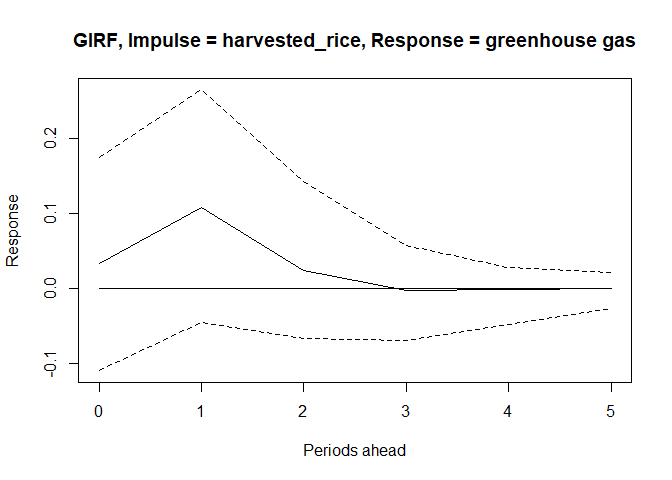
\includegraphics[width=1\linewidth]{pic/IRF Analysis model 1-1.png}
    % \caption{GIRF 1-1}\label{Fig:GIRF 1-1}
   \end{minipage}\hfill
   \begin{minipage}{0.48\textwidth}
     \centering
     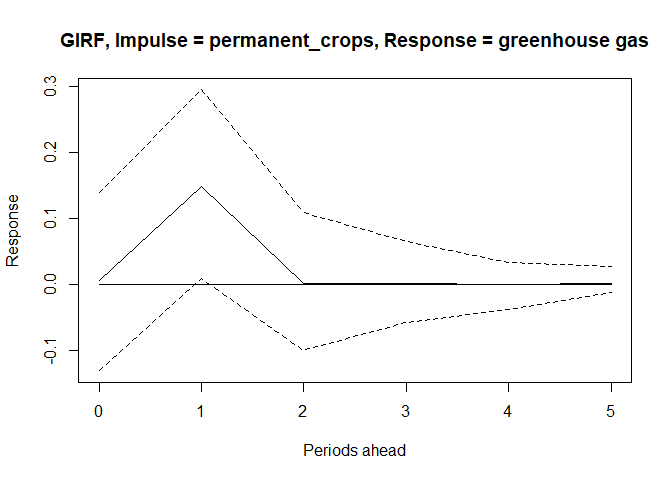
\includegraphics[width=1\linewidth]{pic/IRF Analysis model 1-2.png}
     %\caption{GIRF 1-2}\label{Fig: GIRF 1-2}
   \end{minipage}
\end{figure}
\end{frame}


\begin{frame}{Model 2 $\hat{\beta}$ and $\hat{\Sigma}$}
\begin{table}[H]
\centering
\label{tab:tab_beta_2}
\resizebox{8cm}{!}{
\begin{tabular}{|l|c|c|c|c|c|c|c|c|}
  \hline
 \multirow{Model 2 $\hat{\beta}$} & \multicolumn{2}{c|}{$greenhouse_{t-1}$} & \multicolumn{2}{c|}{$energy\_dep_{t-1}$}  & \multicolumn{2}{c|}{$oil\_imports_{1}$} & \multicolumn{2}{c|}{$const$} \\  \cline{2-9}
 & $\hat{\beta}_{ols}$ & $\hat{\beta}_{B}$ & $\hat{\beta}_{ols}$ & $\hat{\beta}_{B}$ & $\hat{\beta}_{ols}$ & $\hat{\beta}_{B}$ & $\hat{\beta}_{ols}$ & $\hat{\beta}_{B}$\\
  \hline
    $greenhouse_{t}$ & -0.06 & -0.06 & 0.12 & 0.12 & 0.19  &  0.20 &  -0.07  & -0.07  \\ 
    $energy\_dep_{t}$ & 0.14 & 0.14 & -0.51 &  -0.51 & -0.02 & -0.02 &-0.12 & -0.12\\ 
    $oil\_imports_{t}$ & 0.01 & 0.01 & -0.02 & -0.02 & -0.04 & -0.04 & -0.10 & -0.10 \\ 
   \hline
\end{tabular}}
%\caption{Bayesian and OLS estimation of $\hat{\beta}$, Model 2} \label{tab:tab_beta_2}
\end{table}
\\
\begin{table}[H]
\centering
\resizebox{7.5cm}{!}{
\begin{tabular}{|l|c|c|c|c|c|c|c|c|}
  \hline
 \multirow{Model 2 $\hat{\Sigma}$} & \multicolumn{2}{c|}{$greenhouse_{t-1}$} & \multicolumn{2}{c|}{$energy\_dep_{t-1}$}  & \multicolumn{2}{c|}{$oil\_imports_{1}$} \\  \cline{2-7}
 & $\hat{\Sigma}_{ols}$ & $\hat{\Sigma}_{B}$ & $\hat{\Sigma}_{ols}$ & $\hat{\Sigma}_{B}$ & $\hat{\Sigma}_{ols}$ & $\hat{\Sigma}_{B}$ \\
  \hline
    $greenhouse_{t-1}$ & 0.09 & 0.12 & 0.09 & 0.08 & 0.09  &  0.08   \\ 
    $energy\_dep_{t-1}$ & 0.09 & 0.08 & 0.33 &  0.33 & 0.12 & 0.11 \\ 
    $oil\_imports_{t-1}$ & 0.09 & 0.08 & 0.12 & 0.11 & 0.13 & 0.16 \\ 
   \hline
\end{tabular}}
%\caption{Bayesian and OLS estimation of $\hat{\Sigma}$, Model 2} \label{tab:tab_sigma_2}
\end{table}
\end{frame}

\begin{frame}{GIRF, Model 2}
\begin{figure}[!htb]
   \begin{minipage}{0.48\textwidth}
     \centering
     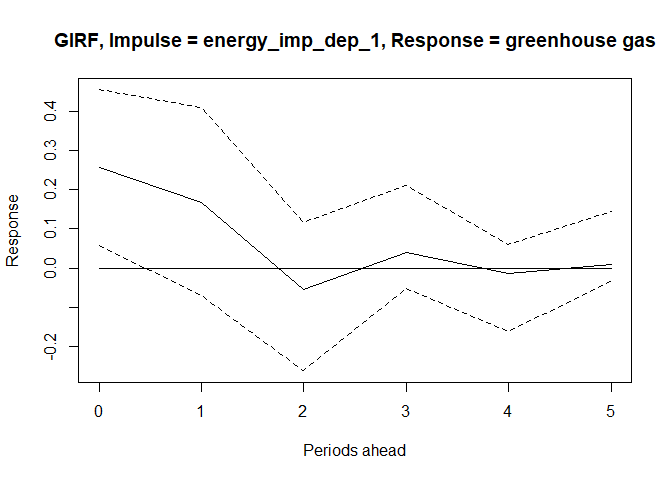
\includegraphics[width=1\linewidth]{pic/IRF Analysis model 2-1.png}
    % \caption{GIRF 2-1}\label{Fig:GIRF 2-1}
   \end{minipage}\hfill
   \begin{minipage}{0.48\textwidth}
     \centering
     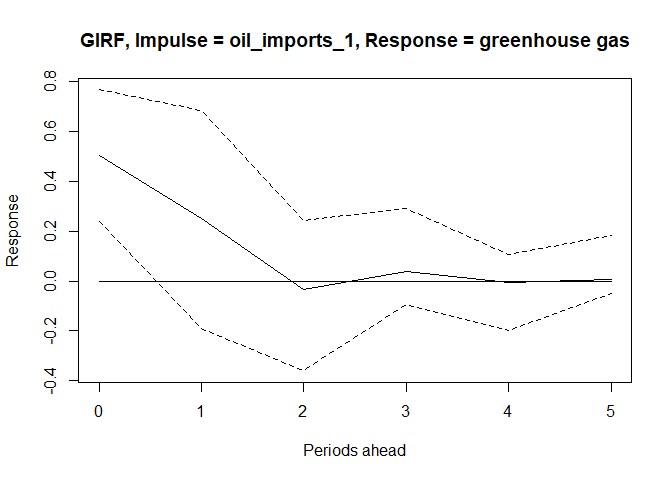
\includegraphics[width=1\linewidth]{pic/IRF Analysis model 2-2.png}
     %\caption{GIRF 2-2}\label{Fig: GIRF 2-2}
   \end{minipage}
\end{figure}
\end{frame}


\begin{frame}{Model 3 $\hat{\beta}$ and $\hat{\Sigma}$}
\begin{table}[H]
\centering
\label{tab:tab_beta_3}
\resizebox{8cm}{!}{
\begin{tabular}{|l|c|c|c|c|c|c|c|c|}
  \hline
 \multirow{Model3 $\hat{\beta}$} & \multicolumn{2}{c|}{$greenhouse_{t-1}$} & \multicolumn{2}{c|}{$GDP_{t-1}$}  & \multicolumn{2}{c|}{$fertilizer_{t-1}$} & \multicolumn{2}{c|}{$const$} \\  \cline{2-9}
 & $\hat{\beta}_{ols}$ & $\hat{\beta}_{B}$ & $\hat{\beta}_{ols}$ & $\hat{\beta}_{B}$ & $\hat{\beta}_{ols}$ & $\hat{\beta}_{B}$ & $\hat{\beta}_{ols}$ & $\hat{\beta}_{B}$\\
  \hline
    $greenhouse_{t}$ & -0.25 & -0.18 & 0.39 & 0.33 & 0.10  &  0.10 &  -0.13  & -0.12 \\ 
    $GDP_{t}$ & 0.17 & 0.19 & 0.17 &  0.14 & 0.01 & 0.01 & 0.03 & 0.03\\ 
    $fertilizer_{t}$ & -0.52 & -0.35 & -0.29 & 0.17 & 0.35 & 0.31 & -0.11 & -0.09 \\ 
   \hline
\end{tabular}}
%\caption{Bayesian and OLS estimation of $\hat{\beta}$, Model 3} \label{tab:tab_beta_3}
\end{table}
\\
\begin{table}[H]
\centering
\resizebox{7.5cm}{!}{
\begin{tabular}{|l|c|c|c|c|c|c|c|c|}
  \hline
 \multirow{Model 3 $\hat{\Sigma}$} & \multicolumn{2}{c|}{$greenhouse_{t-1}$} & \multicolumn{2}{c|}{$GDP_{t-1}$} & \multicolumn{2}{c|}{$fertilizer_{t-1}$} \\  \cline{2-7}
 & $\hat{\Sigma}_{ols}$ & $\hat{\Sigma}_{B}$ & $\hat{\Sigma}_{ols}$ & $\hat{\Sigma}_{B}$ & $\hat{\Sigma}_{ols}$ & $\hat{\Sigma}_{B}$ \\
  \hline
    $greenhouse_{t-1}$ & 0.09 & 0.12 & 0.09 & 0.08 & 0.07  &  0.06   \\ 
    $GDP_{t-1}$ & 0.09 & 0.08 & 0.20 &  0.22 & 0.06 & 0.05 \\ 
    $fertilizer_{t-1}$ & 0.07 & 0.06 & 0.06 & 0.05 & 0.32 & 0.33 \\ 
   \hline
\end{tabular}}
%\caption{Bayesian and OLS estimation of $\hat{\Sigma}$, Model 3} \label{tab:tab_sigma_3}
\end{table}
\end{frame}

\begin{frame}{GIRF, Model 3}
\begin{figure}[!htb]
   \begin{minipage}{0.48\textwidth}
     \centering
     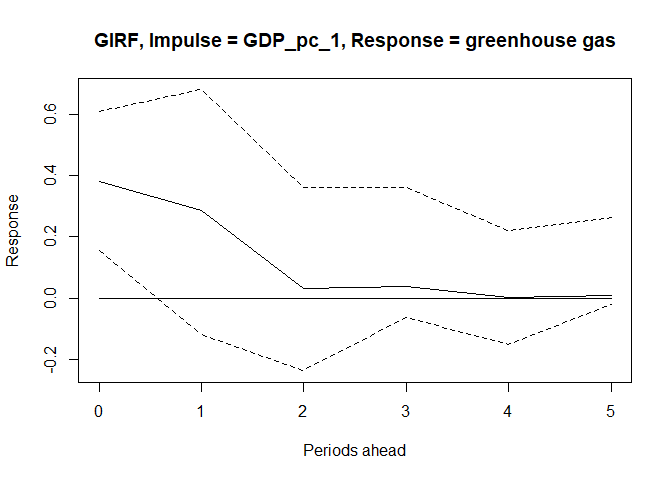
\includegraphics[width=1\linewidth]{pic/IRF Analysis model 3-1.png}
    % \caption{GIRF 3-1}\label{Fig:GIRF 3-1}
   \end{minipage}\hfill
   \begin{minipage}{0.48\textwidth}
     \centering
     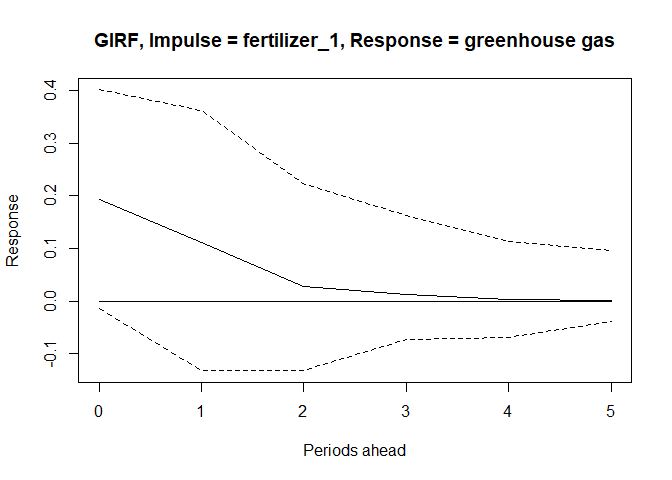
\includegraphics[width=1\linewidth]{pic/IRF Analysis model 3-2.png}
    % \caption{GIRF 3-2}\label{Fig: GIRF 3-2}
   \end{minipage}
\end{figure}
\end{frame}

\begin{frame}{GIRF summary}
\begin{table}[H]
\centering
\resizebox{8cm}{!}{
\begin{tabular}{|c|c|c|c|c|c|c|}
\toprule
 Models & \multicolumn{2}{|c|}{M1} & \multicolumn{2}{|c|}{M2}  & \multicolumn{2}{|c|}{M3} \\ \cline{1-7}
    n-ahead & rice & crops & ener imp & oil imp & gdp pc & fertilizer \\ \hline
    0 & 0.03 & 0.01 & 0.26 & 0.51 & 0.38  &  0.19  \\ 
    1 & 0.11 & 0.15 & 0.17 &  0.25 & 0.29 & 0.11 \\ 
    2 & -0.02 & 0.00 & -0.05 & -0.03 & 0.03 & 0.03  \\ 
    3 & 0.00 & 0.00 & 0.04 & 0.04 & 0.04 & 0.01 \\
    4 & 0.00 & 0.00 & -0.01 & -0.01 & 0.00 & 0.00 \\
    5 & 0.00 & 0.00 & 0.01 & 0.01 & 0.01 &  0.00 \\
 \bottomrule
\end{tabular}}
%\caption{GIRF summary} \label{tab:girf_summary}
\end{table}

\end{frame}

\begin{frame}{FEVD summary}
\begin{figure}
    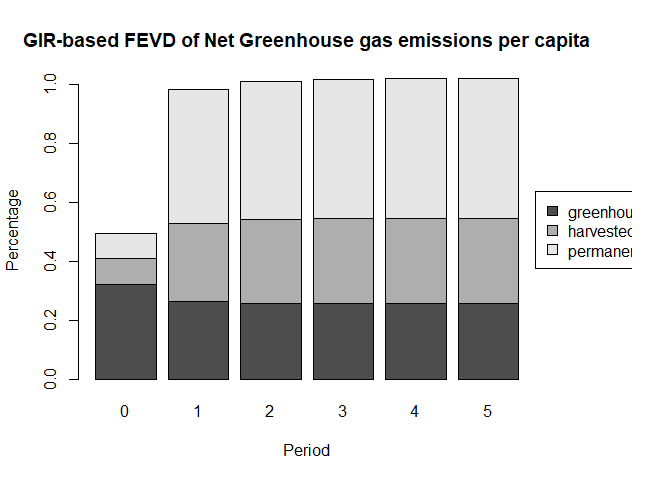
\includegraphics[width=.33\textwidth]{pic/Error Variance Decomposition model 1-1.png}\hfill
    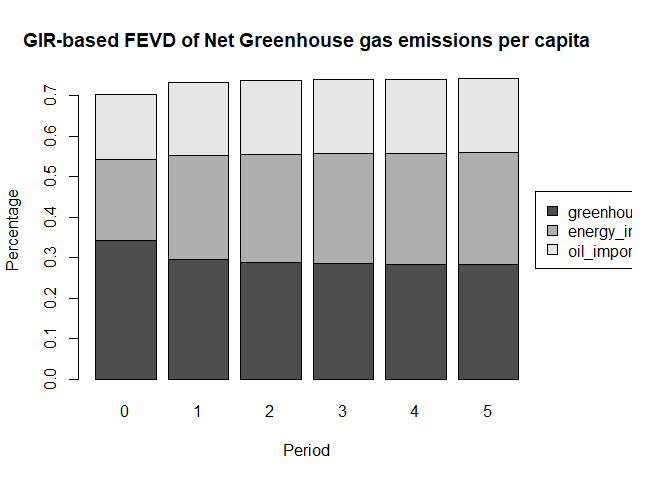
\includegraphics[width=.33\textwidth]{pic/Error Variance Decomposition model 2-1.png}\hfill
    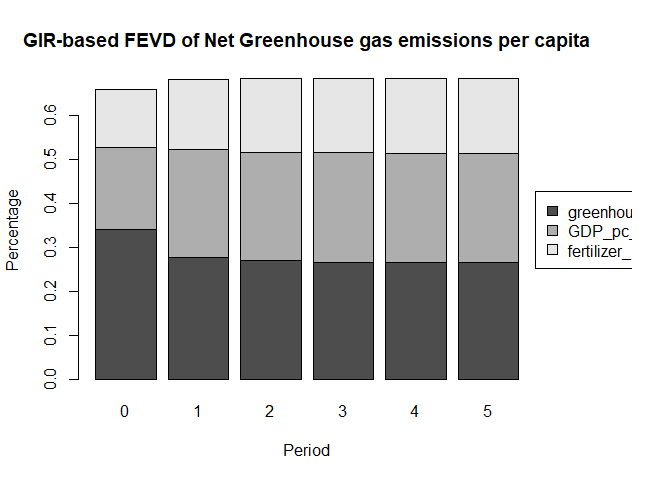
\includegraphics[width=.33\textwidth]{pic/Error Variance Decomposition model 3-1.png}\hfill
    %\\[\smallskipamount]
    %\caption{Some images}
    \label{fig:FEVD Summary}
\end{figure}

\end{frame}

\section{Conclusions}
\begin{frame}{Conclusions and further improvements}
\begin{itemize}
    \item OLS and Bayesian estimate were practically the same
    \item all the modelled variables have a positive increase in greenhouse gases emissions
    \item \textit{oil imports}, \textit{GDP pc} and \textit{energy dependency} are the variables with the higher impact on greenhouse gases emissions
    \item a larger VAR model including all the variables here tested could provide further insights
\end{itemize}
\end{frame}

\appendix

\begin{frame}
    \begin{center}
        {\Huge\calligra Thanks!}
    \end{center}
\end{frame}

\end{document}